\subsection[La libreria \textit{caret} in R]{La libreria \textit{caret} in R}


\begin{frame}
	
	\frametitle{La libreria \textbf{caret} in R per la classificazione e la regressione}
	
	\begin{figure}[!htbp]
		\centering
		
\includegraphics[width=0.85\linewidth]{images/supervised/coding/caret.png}
		%\caption{La libreria \href{https://github.com/topepo/caret}{\textit{caret}} in R}
		
	\end{figure}
	
\end{frame}



\begin{frame}
	
	\frametitle{La libreria \textbf{caret} in R per la classificazione e la regressione}
	
		La libreria \textbf{caret}:
		\begin{itemize}
			\item il nome \textit{caret} deriva dalla abbreviazione di \textbf{C}lassification \textbf{A}nd \textbf{RE}gression \textbf{T}raining
			\pause
			\item contiene funzioni per semplificare il processo di addestramento di modelli per problemi di \textbf{regressione} e \textbf{classificazione} complessi
			\pause
			\item il pacchetto combina altre librerie R ma cerca di non caricarli tutti all'avvio della libreria. Caret carica i pacchetti secondo necessità e presume che siano installati. Se manca un pacchetto di modellazione, viene richiesto di installarlo
			\pause
			\item mette a disposizione una serie di funzioni di alto livello per poter addestrare/valutare/utilizzare vari modelli di machine learning
		\end{itemize}

\end{frame}


\subsubsection[La funzione createDataPartition]{La funzione createDataPartition}
\begin{frame}
	
	\frametitle{La funzione \textbf{createDataPartition}}
	
	
	Innanzitutto, prima di procedere con l'addestramento, è necessario suddividere i dati in due gruppi: un set di addestramento e un set di test.\\\\
	Per fare ciò, possiamo utilizzare la funzione \textbf{createDataPartition}:
		
	\begin{figure}[!htbp]
		\centering
		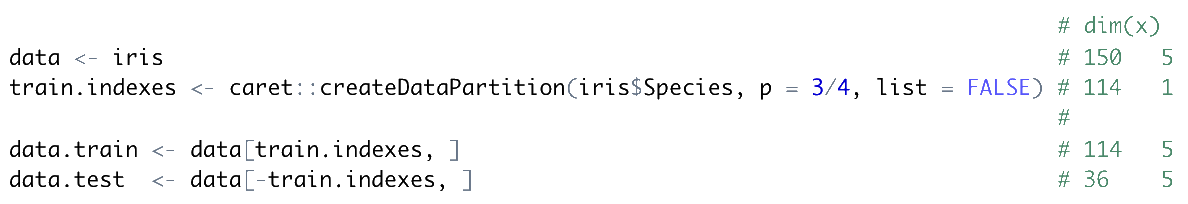
\includegraphics[width=0.9\linewidth]{images/supervised/coding/caret_create_data_partition.png}
		\caption{La funzione createDataPartition della libreria \href{https://github.com/topepo/caret}{\textit{caret}} in R}
	\end{figure}

\end{frame}


\begin{frame}

	\frametitle{Split dei dati: training, validation e test set}
	\begin{columns}
		\column{0.55\linewidth}
		In questo flusso di lavoro quindi si procede nel seguente modo:
		\begin{itemize}
			\item si sceglie il modello che funziona meglio sul validation set (questa operazione viene fatta in automatico da caret)
			\item si ricontrolla il comportamento di quel modello sul test set
		\end{itemize}
		% Questo è un flusso di lavoro migliore perché crea meno esposizioni al set di test.


		\column{0.45\linewidth}
		\begin{figure}[!htbp]
			\centering
			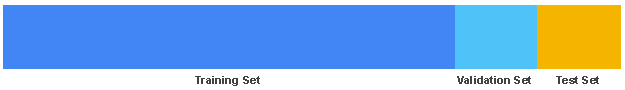
\includegraphics[width=1.0\linewidth]{images/supervised/validation_test_splitting_data/Training_Test_Validation_1.pdf}
			\caption{Split training e test set}
		\end{figure}

		\begin{figure}[!htbp]
			\centering
			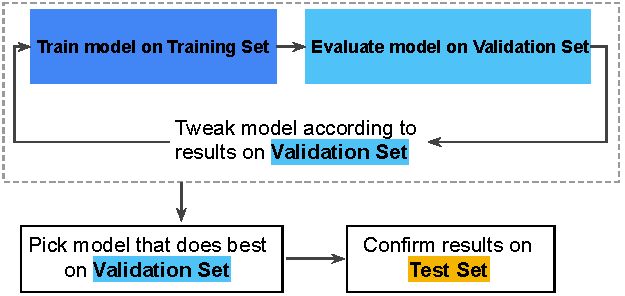
\includegraphics[width=1.0\linewidth]{images/supervised/validation_test_splitting_data/Training_Test_Validation_2.pdf}
			\caption{Workflow training e test set}
		\end{figure}

	\end{columns}
\end{frame}


\subsubsection[La funzione train]{La funzione train}
\begin{frame}
	
	\frametitle{La funzione \textbf{train}}
	
	
	Uno degli strumenti principali nel pacchetto è la funzione \textbf{train} che può essere utilizzata per addestrare un modello.\\\\
	Qualora questo modello sia parametrico la funzione \textbf{train} esplorerà per voi alcune combinazioni di questi parametri alla ricerca della combinazione che ottiene i risultati più promettenti.\\
	
	\begin{figure}[!htbp]
		\centering
		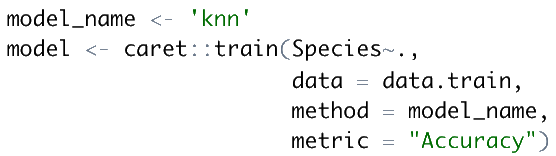
\includegraphics[width=0.75\linewidth]{images/supervised/coding/caret_train_1.png}
		\caption{La funzione train della libreria \href{https://github.com/topepo/caret}{\textit{caret}} in R}
	\end{figure}

\end{frame}



\begin{frame}

	\frametitle{Workflow con training, validation e test set}
	\begin{figure}[!htbp]
		\centering
		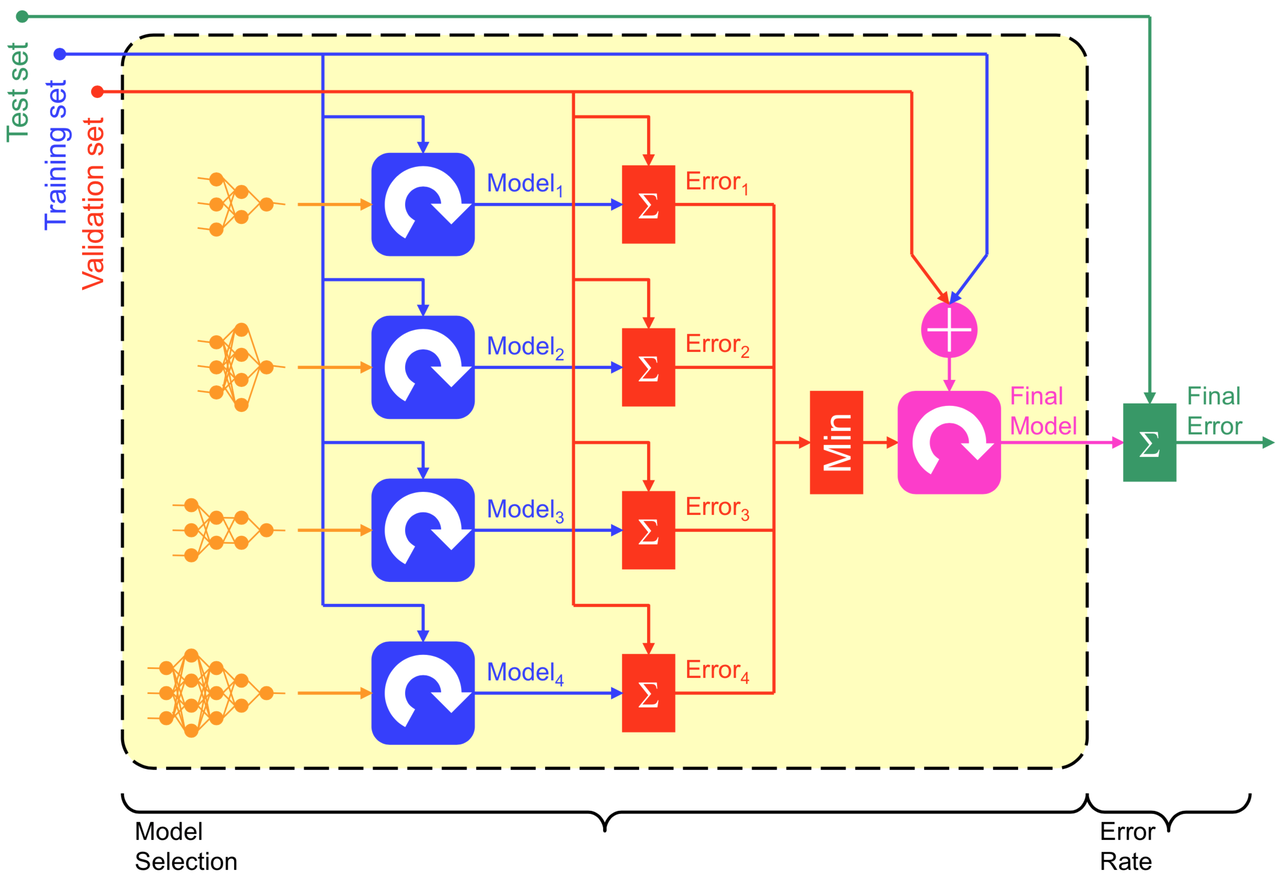
\includegraphics[width=0.85\linewidth]{images/supervised/validation_test_splitting_data/Workflow.png}
%		\caption{Split training e test set}
	\end{figure}
\end{frame}




\begin{frame}
	
	\frametitle{La funzione \textbf{train}}
	
	
	La libreria \textbf{caret} mette a disposizione una serie molto ampia di modelli.\\\\
	Con lo stesso metodo \textbf{train} è possibile addestrare diverse tipologie di modelli semplicemente andando a cambiare il valore passato come \textbf{method}.\\
	
	\begin{figure}[!htbp]
		\centering
		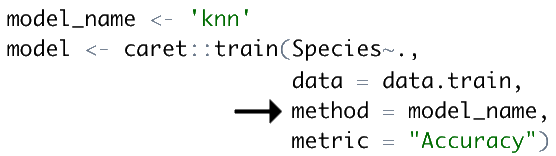
\includegraphics[width=0.75\linewidth]{images/supervised/coding/caret_train_2.png}
		\caption{La funzione train della libreria \href{https://github.com/topepo/caret}{\textit{caret}} in R}
	\end{figure}

\end{frame}


\begin{frame}
	
	\frametitle{La funzione \textbf{train}}
	
	
	Per una lista completa dei possibili modelli consultare i seguenti links:
	\begin{itemize}
		\item \href{https://topepo.github.io/caret/available-models.html}{\textit{available-models}}
		\item \href{http://topepo.github.io/caret/train-models-by-tag.html}{\textit{train-models-by-tag}}
	\end{itemize}
	~\\
	Alcuni dei modelli di classificazione e regressione che abbiamo studiato possono essere utilizzati all'interno di caret:
	
	\begin{figure}[!htbp]
		\centering
		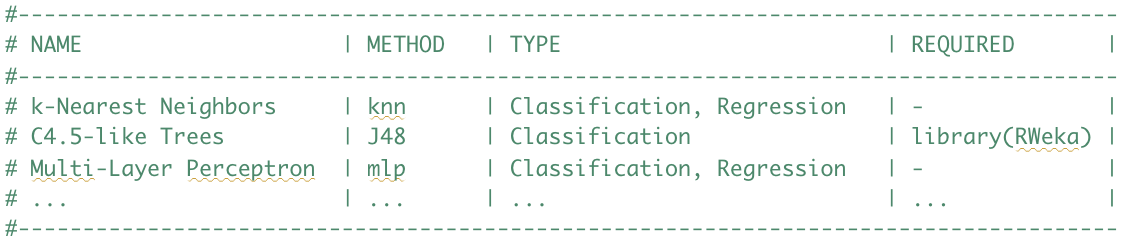
\includegraphics[width=1.0\linewidth]{images/supervised/coding/caret_models.png}
		\caption{Alcuni modelli della libreria \href{https://github.com/topepo/caret}{\textit{caret}} in R}
	\end{figure}

\end{frame}


\subsubsection[La funzione predict]{La funzione predict}
\begin{frame}
	
	\frametitle{La funzione \textbf{predict}}
	
	
	Una volta costruito il modello con la funzione \textbf{train} possiamo effettuare la predizione usando il metodo \textbf{predict} (appartenente alla libreria	 \textbf{stats} precaricata in automatico da R).\\\\
	Si può utilizzare \textbf{predict} per ottenere la predizione più probabile o per ottenere le probabilità associata a ciascuna classe.
	
	\begin{figure}[!htbp]
		\centering
		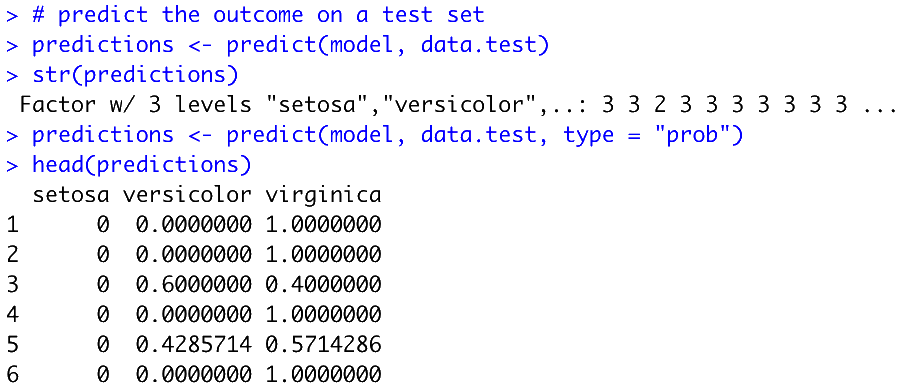
\includegraphics[width=0.70\linewidth]{images/supervised/coding/caret_predict.png}
		\caption{La funzione predict in R}
	\end{figure}

\end{frame}


\subsubsection[La funzione confusionMatrix]{La funzione confusionMatrix}
\begin{frame}
	
	\frametitle{La funzione \textbf{confusionMatrix}}
	
	
	Una volta ottenute le predizioni per un certo testing set si può utilizzare la funzione \textbf{confusionMatrix} per ottenere una panoramica della efficacia della predizione confrontando tra loro il risultato predetto con quello atteso.
	
	\begin{figure}[!htbp]
		\centering
		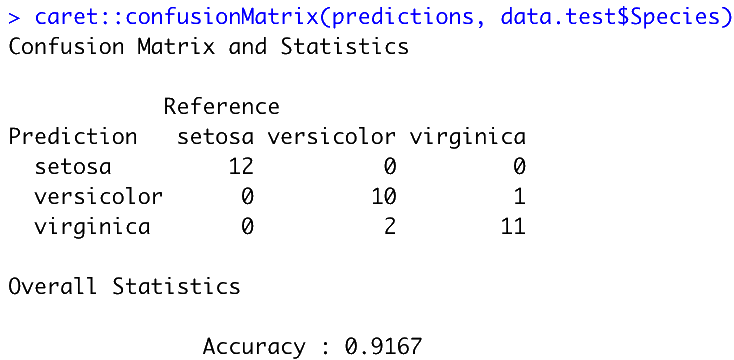
\includegraphics[width=0.75\linewidth]{images/supervised/coding/caret_confusion_matrix.png}
		\caption{La funzione confusionMatrix della libreria \href{https://github.com/topepo/caret}{\textit{caret}} in R}
	\end{figure}

\end{frame}